% Source: Code/xband-radar-sim/docs/radar_simulation_technical.tex
% Description: Phasor representation of echoes at different ranges. The phase rotates rapidly with range due to the short wavelength.

\documentclass[border=4pt]{standalone}
\usepackage{algpseudocode}
\usepackage{amsmath,amssymb,amsfonts}
\usepackage[T1]{fontenc}
\usepackage{graphicx}
\usepackage{pgfplots}
\usepackage{tikz}
\usepackage{xcolor}
\pgfplotsset{compat=1.18}
\usetikzlibrary{arrows.meta,positioning,shapes.geometric,calc,patterns,decorations.pathmorphing,3d,angles,quotes}

\definecolor{radargreen}{RGB}{0,255,0}
\definecolor{raycolor}{RGB}{255,165,0}
\definecolor{targetcolor}{RGB}{255,0,0}
\definecolor{groundcolor}{RGB}{139,90,43}
\definecolor{skycolor}{RGB}{135,206,235}
\definecolor{beamcolor}{RGB}{255,255,0}


\begin{document}
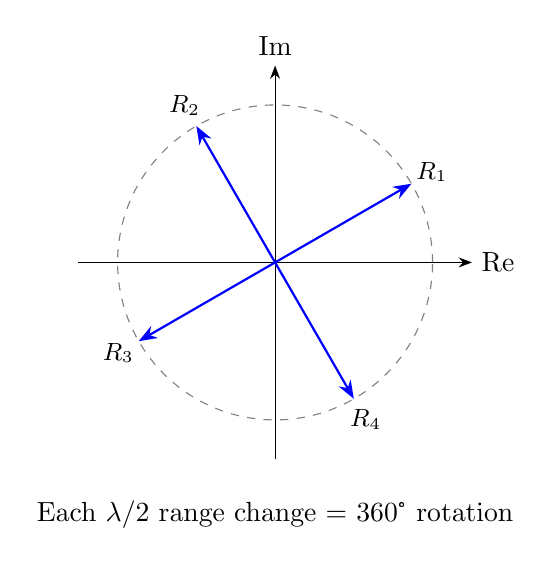
\begin{tikzpicture}
    % Phasor diagram
    \draw[-{Stealth}] (-2.5,0) -- (2.5,0) node[right] {Re};
    \draw[-{Stealth}] (0,-2.5) -- (0,2.5) node[above] {Im};

    % Unit circle
    \draw[gray, dashed] (0,0) circle (2);

    % Multiple phasors at different ranges
    \foreach \angle/\label in {30/R_1, 120/R_2, 210/R_3, 300/R_4} {
        \draw[-{Stealth}, thick, blue] (0,0) -- ({2*cos(\angle)},{2*sin(\angle)});
        \node at ({2.3*cos(\angle)},{2.3*sin(\angle)}) {\small $\label$};
    }

    \node at (0,-3.2) {Each $\lambda/2$ range change = 360° rotation};
\end{tikzpicture}
\end{document}
